Nachdem die grundsätzliche Idee, Prinzipien und die etablierte Kultur von DevOps beschrieben worden sind, wird in diesem Absatz näher auf die inhaltlichen Aspekte von DevOps eingegangen.

Der DevOps-Lebenszyklus besteht aus einer aus mehreren iterativen und häufig automatisierten Workflows, die innerhalb eines größeren, iterativen und automatisierten Zyklus ausgeführt werden.

Grundsätzlich baut der Entwicklungszyklus innerhalb einer DevOps-Umgebung auf sieben Phasen auf, wie in der unteren Abbildung zu erkennen ist.

Der DevOps-Zyklus verläuft stets in einer Schleife, wodurch sowohl der Prozess als Ganzes als auch die Phasen sich untereinander durchgehend wiederholen, um eine stetige Neuimplementierung, Weiterentwicklung, Zusammenarbeit und Feedback sicherzustellen. 

Aufgrund der Iteration es Zykluses können Fehler in den einzelnen Phasen frühzeitig erkannt und beiseitigt werden und tragen zur Verbesserung der gesamten Phase bei. 

Die Abbildung zeigt die Abgrenzung zwischen den Mitgliedern des Development- und den Operationsteam.

Jede Seite trifft einerseits auf seperate und andererseits auf ständig zusammenarbeitende Teams zum Ziel die Geschwindigkeit, Zuverlässigkeit und die Qualität des Prozesses zu gewährleisten. 

\begin{figure}[h]
    \centering
    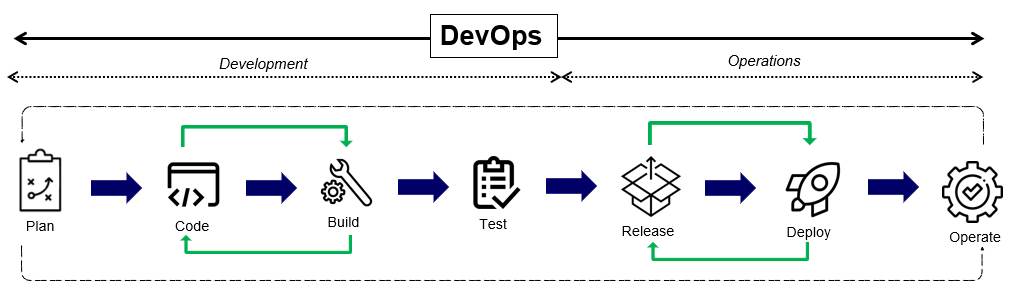
\includegraphics[scale=0.6]{Bilder/DevOps Lebenszyklus.png}
    \caption{Entwicklungszyklus innerhalb einer DevOps-Umgebung, angelehnt an \cite[S. 16]{halstenberg_devops_2020}}
\end{figure}

\paragraph{Plan}

In dieser Phase werden zunächst die wesentliche Anforderungen anhand der Bedürfnisse aller Stakeholder oder durch erhaltenes Feedback festgelegt, mit dem Ziel die Entwicklung und die Auslieferung entsprechend zu planen. \cite[s. 16]{halstenberg_devops_2020}  

Hinzu kommen die definierten Problembeschreibungen als auch der Umfang. 

Ziel ist es die entsprechenden Ressourcen und die Entwicklungen während des ganzen Zeitraums zu planen und einzuteilen. 

Darüber hinaus können Entwickler sich einen Überblick über die Verwendung von Systemen, Features, Funktionalitäten Risiken und Einschränkungen verschaffen. \cite{yarlagadda_devops_2021} 

Auch die Durchführbarkeit und Machbarkeit wird über den gesamten Zeitraum besprochen und geplant. 

Innerhalb dieser Phase kommen Methoden der agilen Softwareentwicklung wie Scrum, Kanban oder Extreme Programming zum Einsatz.

So kann mittels eines Kanban-Boards jeder Arbeitsschritt angefangen bei einem definierten Zustand bis zur Erledigung dieser Aufgabe, anhand vertikalen Lanes als mögliche Zustände, als Karte bewegt werden. \cite[S. 88]{huttermann_devops_2012}  

Durch die Planung und Koordination mittels Kanban-Board können nicht reine Entwicklungstätigkeiten, sondern auch Schwerpunkte im Hinblick auf den Betrieb zur Infrastruktur oder Wartung abgebildet werden. \cite{schaefer_devops_2017} 

In diesem Zuge können Schwachstellen und Engpässe schnell aufgedeckt werden, wodruch der gesamte Prozessfluss optimiert wird. 

Zur kurzfristigen Kontrolle können die auf Scrum basierenden Planungsgrundsätze verwendet werden, da dieses auf zeitlich begrenzte Iterationen und die Verteilung von Rollen und Zuständigkeiten setzt.

Im Rahmen von Scrum werden zunächst alle am System zu erledigenden Arbeiten im 'Release Backlog' festgehalten. 

Während der Planung für den Sprint werden Features und Funktionen aus dem Release Backlog ausgewählt und in das 'Sprint-Backlog' oder nach Prioritäten gesetzten Aufgaben aufgenommen, die im nächsten Sprint abgeschlossen werden sollen. \cite{cohen_introduction_2004}

Infoldessen können mögliche Entwicklungsaufwände auf einen zeitlichen Umfang versehen ('Timeboxing'). \cite[s. 17]{halstenberg_devops_2020}

Die Organisation des Teams findet in kleinen Sitzungen und monatlichen Sprints oder Iterationen statt. 

Wichtige Gemeinsamkeit beider Methoden ist die Arbeit nach dem Pull-Prinzip, wobei Tasks eigenständig bearbeitet werden, wenn die entsprechende Kapazität zur Verfügung steht. \cite{concas_agile_2007} 

Der Hauptunterschied zwischen beiden Methoden besteht im wesentlichen in der Zielsetzung und des zeitlichen Horizonts. 

Während Scrum sich auf die iterative Produktentwicklung konzentiert und das Produkt von Teration zu Iteration erweitert und verbessert, arbeitet die Kanban-Methode auf die kontinuierliche Verbesserung der Prozesse, kürzere Vorlaufzeiten und Vermeidung von Verschwendung, hin. \cite{concas_agile_2007}

Zudem legt Scrum den aktuellen Arbeitsfortschritt und die Planung auf die folgenden Sprints fest, während sich die Planung bei Kanban auf mehrere Wochen bezieht. \cite[s. 5]{verona_practical_2016} 

Insbesondere die messbaren und eindeutigen Vorteile von DevOps zeigen sich innerhalb kürzerer Zyklen, die wiederum die längeren Zyklen effizienter machen. 

\paragraph{Code und Build}

Nachdem die wesentlichen Aufgaben zugewiesen worden sind, stellt die hautpsächliche Akitivität innerhalb dieser Phase die Entwicklung dar. 

Störende Schritte wie beispeilsweise das Testen, die Inbetriebnahme oder die Berücksichtigung der Anfoderungen sollten in dieser Phase bereits berücksicht sein. \cite[S. 18]{halstenberg_devops_2020}  

Die Forschritte des entwickeltenden Programmcode werden laufend in Sprint Reviews, Daily Scrum Meetings kommuniziert an das gesamte DevOps-Team kommuniziert. 

Um eine einheitliche Basis zu schaffen, arbeiten alle Entwicklerteams mit gemeinsamen Tools und Plugins und legen einheitliche Vorgaben für die Qualität des Quellcodes fest. 

Nachdem die Aufgabe abgeschlossen ist, wird der neu entwickelte und lauffähige Programmcode in kleinen Bestandteilen an ein Versionsverwaltungstool ('Code Repository') übergeben.\cite[S. 18]{halstenberg_devops_2020}  

Diese Vorgehensweise wird auch als Push bezeichnet, der wiederrum einen Pull-Request auslöst. 

In diesem Zusammenhang erfolgt ein Code-Review, bei dem der Pull-Request bestätigt wird sobald der Quellcode den Anforderungen funktional entspricht.

Analog zum Pull-Request finden automatisierte Testfälle und die (ausführbare) Konfguration der Test- und Produktionsumgebung statt. \cite[S. 18]{halstenberg_devops_2020}  

Ist das Testen erfolgreich durchlaufen, kann der Quellcode übernommen werden. 

Zudem werden alle Veränderungen am Programmcode, neue Entwicklungen oder Fehleranfälligkeiten dokumentiert und für das gesamte DevOps-Team zur Verfügung gestellt.

\paragraph{Test}

Neben der Entwicklungsphase erfolgt innerhalb der DevOps-Zyklen eine intensive Testphase, die in einer eigenen Ungebung durchgeführt wird und sich vor den Phasen der Intergration und der Bereitstellung befindet. 

Während dieser Phase werden intensive Tests der Anwendungen und Funktionalitäten innerhalb einer eigenen Serverumgebung durchlaufen, die auch als 'Staging Environment' bezeichnet werden. \cite[S. 16]{verona_practical_2016} 

Dabei wird eine Umgebung geschaffen, die sich ähnlich der Produktionsvariante verhält, auf die die finale Version bereitgestellt wird und daher ein Testen unter annährend realen Bedingungen erlaubt. \cite[S. 5.2/5.6]{bass_devops_2015}

Durch die Verwendung von realen Daten sollen Funktionaliäten einerseits unter Berücksichtigung der Infrastruktur geprüft und andererseits simuliert werden, wie sich das System unabhängig von der Entwicklungsumgebung verhält. \cite[S. 16]{verona_practical_2016} 

Während die Entwicklerteams Unit- und Integrationstests durchführen, beteiligt sich der Betrieb an Integrations- und Lasttests, um die Betriebsbereitschaft zu beurteilen. \cite[S. 127]{sturm_devops_2017}  

Neben den automatisierten Tests finden darüber hinaus auch manuelle Tests statt, um Schachstellen oder Risiken in Bereichen wie Sicherheit innerhalb der Anwendung zu identifizieren und zu beseitigen.

\paragraph{Release und Deploy}

Die Phase des Release beschreibt den Prozess der Vorbereitung für die Bereitstellung des Builds an entwickelten Funktionalitäten in die produktive Umgebung. \cite[S. 20]{halstenberg_devops_2020} 

Innerhalb dieser Phase entscheidet sich welche Änderung in dem Release enthalten sein soll. 

Abhängig des Fortschrittes des Release-Prozesses kann die Übergabe sowohl manuell oder automatisch erfolgen, wobei Entwickler die Möglichkeit haben, Funktionalitäten für den Kunden zu deaktivieren bis diese einsatzbereit sind. \cite{thedev_eight_2019}

In diesem Zuge können neue Versionen innerhalb fester Zeiträume erfolgen oder automatisiert, nach erfolgreicher Übergabe des Quellcodes durch die Testphase. \cite{thedev_eight_2019}

Innerhalb der Phase des Deploys findet das eigentliche Ausrollen des neuen Builds statt.  

Grundsätzlich kann dieser Schritt automatisiert durchgeführt werden, damit es keine Einschränkungen des laufenden Betriebs gibt. \cite{thedev_eight_2019}  

Bei Problemen innerhalb des Deployments, kann der letzte Stand aus der Produktivumgebung wiederhergestellt werden, indem die neue Umgebung parallel zur bestehenden Produktionsumgebung aufgebaut wird. 

Häufig kann die Phase des Deploys mit der Phase des Releases übereinstimmen, obwohl diese Phase im Wesentlichen nur die Auslieferung der getesteten Software in die Produktivumgebung beschreibt. \cite[S. 20]{halstenberg_devops_2020}   

Im Rahmen dieser Phase sind zwei grundlegende Rollen verbreitet. \cite[s. 20]{halstenberg_devops_2020} 

Zum einen trifft der Release Coordinator die Entscheidungen über den Produktiveinsatz eines Releases und überwacht den Entwicklungsfortschritt. 

Zum anderen überwacht der Site Reliability Engineer die IT-Services, die notwendigen Tools und Abhängigkeiten innerhalb der Inbetriebnahme des Releases. 

\paragraph{Operate}

Diese Phase beschäftigt sich hauptsächlich um die Wartung und den Support, nachdem die Änderungen live gegangen sind. 

In diesem Rahmen werden einerseits Lastspitzen oder Tiefpunkte anhand der aktiven Nutzerzahl automasiert und effektiv abgefangen und andererseits benötigte Ressourcen zur Verfügung gestellt, um die Produktivumgebung erfolgreich zu betreiben. \cite{thedev_eight_2019}    

Zudem kann der Kunde Feedback zu geben, welches gesammelt und ausgewertet wird, um das Nutzerverhalten der User besser zu verstehen und die zukünftige Entwicklung zu verbessern. 

Häufig wird als finale Phase, die Monitor-Phase zusätzlich in den DevOps-Lebenszyklus aufgenommen, wobei diese oftmals in die Operate-Phase mitaufgenommen werden kann.

Dabei handelt es sich neben dem Kundenfeedback, um die Erhebung von weiteren Daten wie den auftretenden Fehlern, Leistungsverhalten, Zugriffszahlen oder Kapazitäten. \cite{thedev_eight_2019}    

Die erhobenen Informationen werden an die Produktmanager und die Entwicklungsteams oder iterativ an die Planungsphase weitergeleitet, um das nächste Feature am User abzuleiten. \cite[s. 21]{halstenberg_devops_2020} 

Damit kann sichergestellt werden, dass der aktuelle Zustand einer Anwendung überwacht und verwaltet wird, um sich auf Änderungen vorzubereiten und etwaige Fehler zu beheben. \cite[S. 127]{sturm_devops_2017} \\

















 






















%Nun wurde die Idee hinter dem DevOps-Ansatz wird in den vorherigen Kapiteln beschrieben. Als nächstes soll nun näher auf die inhaltlichen Themen von DevOps eingegangen werden, sowie der DevOps Life Cycle und dessen Phasen. Damit der Life Cycle nicht zu weitgreifend wird, wird lediglich der Life Cycle, der bei der msg systems ag verwendet wird, näher beschrieben. Damit sollte der Leser ein Verständnis für die weiteren Punkte im Proof Of Concept erlangen.\\




%Gemäß Fluri u.a. \cite[S. 259 - 283]{tokarski_strategische_2018} muss ein optimaler DevOps-Prozess drei Voraussetzungen erfüllen, um erfolgreich etabliert zu werden. Erste Voraussetzung bilden zunächst die \textit{automatisierten und definierten Prozesse}. Um Prozesse optimiert und effizient zu etablieren und zu automatisieren, bedarf es zunächst einer umfassenden Definition über die Funktionsweise und den Ablauf dieses Prozesses. Hinzu kommt eine \textit{integrierte Infrastruktur(Toolchain)}. Anhand technischer Komponenten als geeignete Werkzeuge, die dem DevOps-Team zur Verfügung gestellt werden, kann die Automatisierung optimal abgebildet werden. Letzte grundsätzliche Voraussetzung stellt das \textit{Rahmenwerk von Aktivitäten für die Teams} auf. Diese Voraussetzung zielt auf die Etablierung einer DevOps-Kultur, die bereits im vorherigen Kapitel dargestellt wurde. Gemäß Fluri u.a. \cite[S. 259 - 283]{tokarski_strategische_2018} wird der gesamte Entwicklungszyklus in DevOps durch acht Schritte und vier Prozessgebiete abgebildet. 